\documentclass{article}
\usepackage{tikz}
\usepackage{xcolor}
% Make sure ALL needed libraries are loaded
\usetikzlibrary{positioning, arrows.meta, shapes.geometric, fit, backgrounds, calc} 

% Define custom colors
\definecolor{lightgreen}{RGB}{200, 230, 200}
\definecolor{lightblue}{RGB}{173, 216, 230} % Standard light blue
\definecolor{lighterblue}{RGB}{211, 225, 245} % Even lighter blue for projection
\definecolor{lightpink}{RGB}{245, 200, 195} % Salmon/coral color

\begin{document}

\begin{figure}[htbp] % Added placement specifier [htbp]
\centering
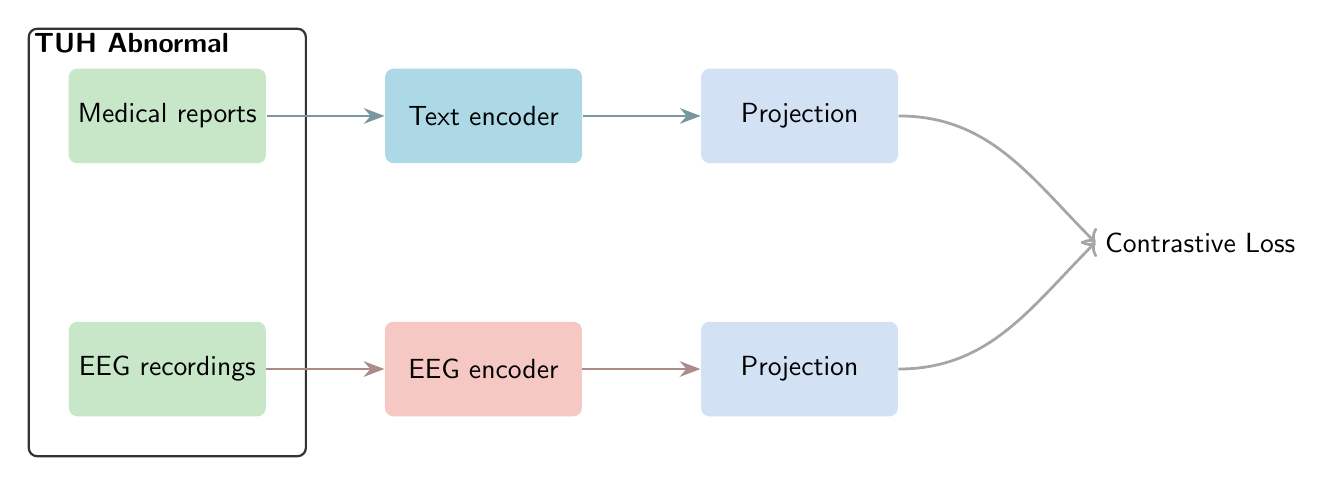
\begin{tikzpicture}[
    node distance=1cm, % Base node distance (can be overridden)
    box/.style={ % Style for main boxes, takes fill color as argument
        rectangle,
        rounded corners=3pt, % Slightly smaller rounding
        minimum width=2.5cm,
        minimum height=1.2cm, % Adjusted height slightly
        text centered,
        font=\sffamily,
        draw=none, % No border, fill provides shape
        fill=#1
    },
    % Specific styles using the base 'box' style
    input/.style={box=lightgreen},
    text_encoder/.style={box=lightblue, text=black}, % Specify text color if needed
    eeg_encoder/.style={box=lightpink, text=black},  % Specify text color if needed
    projection/.style={box=lighterblue},
    % Arrow style
    arrow/.style={
        -Stealth, % Arrow tip style
        thick,
        line width=1pt,
        draw=#1 % Make arrow color an argument
    },
    % Default arrow color (if not specified later)
    arrow/.default=black 
]

% Input blocks
\node[input] (medical) {Medical reports};
\node[input] (eeg) [below=2.0cm of medical] {EEG recordings}; % Adjusted spacing

% Encoder blocks
\node[text_encoder] (text_enc) [right=1.5cm of medical] {Text encoder};
\node[eeg_encoder] (eeg_enc) [right=1.5cm of eeg] {EEG encoder};

% Projection blocks
\node[projection] (proj1) [right=1.5cm of text_enc] {Projection};
\node[projection] (proj2) [right=1.5cm of eeg_enc] {Projection};

% Draw arrows (Pass color to the arrow style)
% Using slightly darkened versions of the fill colors for arrows
\draw[arrow=lightblue!70!black] (medical) -- (text_enc); 
\draw[arrow=lightblue!70!black] (text_enc) -- (proj1);
\draw[arrow=lightpink!70!black] (eeg) -- (eeg_enc);
\draw[arrow=lightpink!70!black] (eeg_enc) -- (proj2);

% Contrastive Loss text and arrows
% *** THE FIX IS HERE *** Combine options into one [...] block
\node[font=\sffamily, right=2.5cm of $(proj1.east)!0.5!(proj2.east)$] (loss) {Contrastive Loss}; % Position relative to east anchors for better alignment

% Use slightly curved arrows pointing towards the 'loss' node
\draw[arrow=gray!70, ->] (proj1.east) to [out=0, in=135] (loss.west); % Nicer curve using 'to'
\draw[arrow=gray!70, ->] (proj2.east) to [out=0, in=225] (loss.west); % Nicer curve using 'to'

% Outer container box using background layer and label
% Make sure 'backgrounds' library is loaded
\begin{pgfonlayer}{background}
    \node[
        draw=black!80, % Slightly softer black border
        thick, 
        rectangle, 
        rounded corners=3pt, % Match node rounding
        inner sep=0.5cm, % Padding inside box
        fit=(medical) (eeg), % Fit around these nodes
        label={[font=\sffamily\bfseries, anchor=north west, inner sep=2pt]north west:TUH Abnormal} % Use label option
    ] (tuh) {}; 
\end{pgfonlayer}

\end{tikzpicture}
\caption{Architecture of EEG-CLIP}
\label{fig:eeg-clip}
\end{figure}

\end{document}